\documentclass[letterpaper,headings=standardclasses]{scrartcl}

\usepackage[margin=1in,includefoot]{geometry}
\usepackage{amssymb}
\usepackage{amsmath}
\usepackage{listings}
\usepackage{tikz}
\usepackage{float}

\usetikzlibrary{shapes,arrows}

\tikzset{
  block/.style    = {draw, thick, rectangle},
  sum/.style      = {draw, circle},
  input/.style    = {coordinate, circle},
  output/.style   = {coordinate, circle},
  neuron/.style   = {draw, thick, circle}
}

\lstset{basicstyle=\ttfamily,language=python,columns=flexible,breaklines=true}

\title{Homework 2}
\subtitle{CS 559 - Neural Networks - Fall 2019}
\author{Matteo Corain 650088272}

\begin{document}

\maketitle

\section{Question 1}

\subsection{General architecture of the network}

In order to design a network capable of implementing the proposed separation, it is possible to proceed as follows:

\begin{itemize}

\item First, we need to identify the inequalities that describe the two regions and implement them using a set of perceptrons;

\item Then, since the inequalities for the two regions should be all satisfied at once, we need to connect the outputs of all perceptrons useful for describing a region using a perceptron implementing a logical AND;

\item Finally, since the output of the network should be positive in case the pattern belongs to any of the two regions, we need to connect the outputs of the AND perceptrons using a perceptron implementing a logical OR.

\end{itemize}

Let us first begin to identify the linear relationships that are necessary to identify the colored regions. Using the nomenclature shown in figure \ref{region_names}, we have:

\begin{figure}[h]
\centering
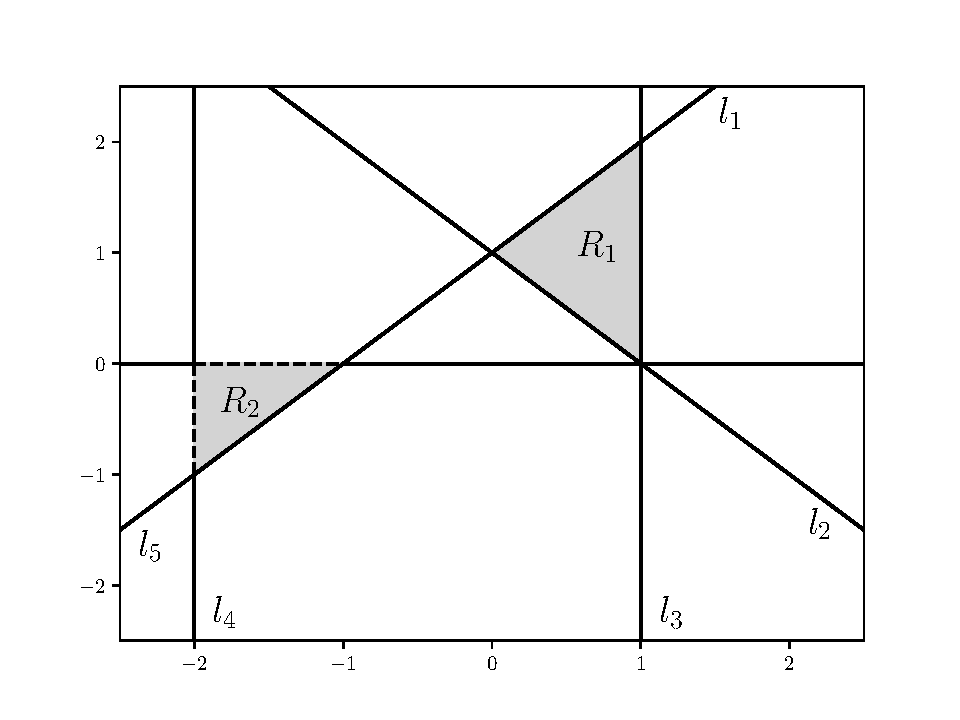
\includegraphics[width=.7\linewidth]{region_names.pdf}
\caption{Nomenclature used for lines and regions}
\label{region_names}
\end{figure}

$$ l_1 : - 1 - x + y = 0, \quad l_2 : -1 + x + y = 0 $$
$$ l_3 : -1 + x = 0, \quad l_4: 2 + x = 0, \quad l_5 : y = 0 $$

Given this nomenclature, the two regions are described by the following set of inequalities:

$$ R_1 = \begin{cases} l_1 \le 0 \\ l_2 \ge 0 \\ l_3 \le 0 \end{cases}, \quad R_2 = \begin{cases} l_1 \ge 0 \\ l_4 > 0 \\ l_5 < 0 \end{cases} $$

As it can be seen, some of these inequalities do not present the equality sign; since the perceptrons we are designing use the step activation function (which returns 1 when the pattern is on the separator), this means that those cannot be implemented by a single perceptron. Instead, we have to make use of a succession of two perceptrons, the first implementing the complimentary inequality and the second implementing a logical NOT:

$$ l_4 > 0 \Rightarrow \neg (l_4 \le 0), \quad l_5 < 0 \Rightarrow \neg (l_5 \ge 0) $$

The block diagram of the network to implement is shown in figure \ref{blk_diagram}; each block represents a perceptron to be designed. As we can see, the network is composed of four distinct layers:

\begin{itemize}

\item The first layer is the \emph{line layer}, and includes the neurons used to implement the separation described by the linear inequalities;

\item The second layer is the \emph{NOT layer}, and includes the neurons used to implement the NOT operation as requested by inequalities not including the equality sign; for inputs that do not need the usage of a NOT perceptron, we can imagine that those are connected to a buffer perceptron, simply returning as output the input value;

\item The third layer is the \emph{AND layer}, and includes the neurons used to implement the AND operation among inequalities useful to describe the same region (all should be satisfied at the same time);

\item The fourth layer is the \emph{OR layer}, and includes the neuron used to implement the OR operation among the results of the previous layer (we want a positive result if the pattern is either in $R_1$ or in $R_2$).

\end{itemize}

\begin{figure}[H]
\centering
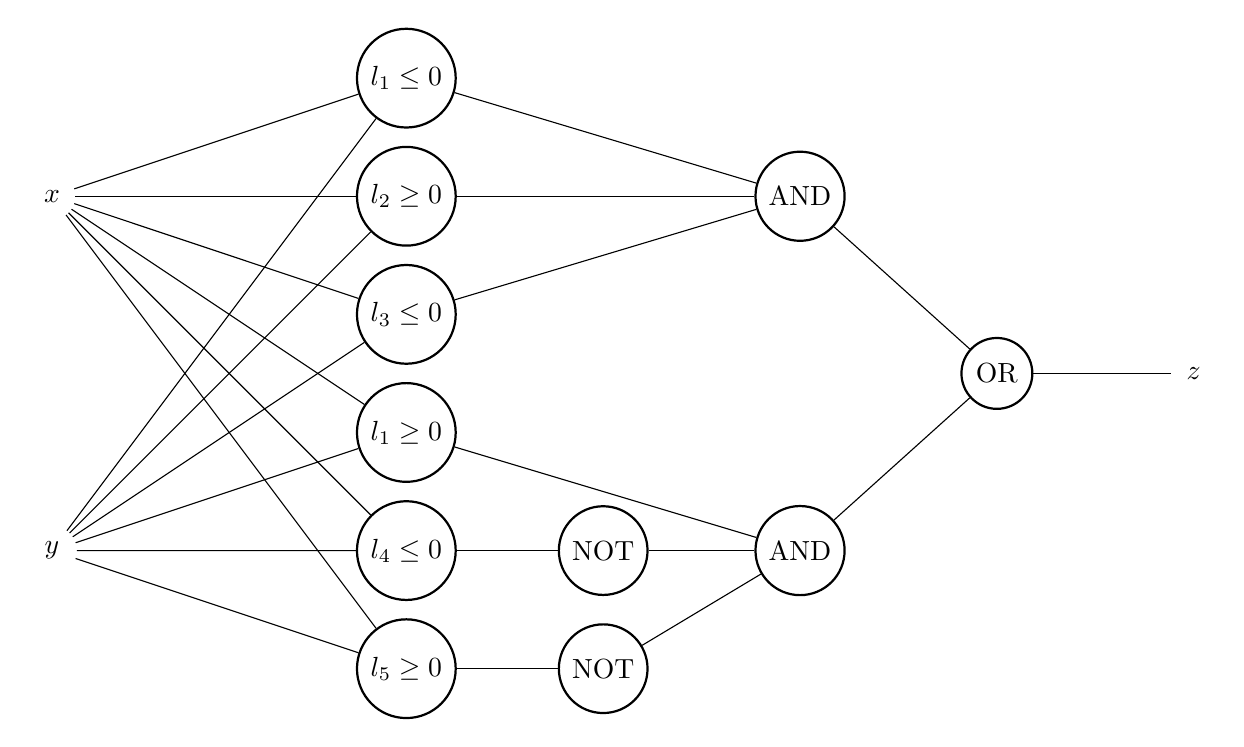
\begin{tikzpicture}[auto, node distance=1.5cm, >=triangle 45]

% Input layer
\draw node [input, name=x] {$x$};
\draw node [input, name=y, below of=x, node distance=4.5cm] {$y$};

% First layer
\draw node [neuron, right of=x, yshift=1.5cm, node distance=4.5cm] (p11) {$l_1 \le 0$};
\draw node [neuron, below of=p11] (p12) {$l_2 \ge 0$};
\draw node [neuron, below of=p12] (p13) {$l_3 \le 0$};
\draw node [neuron, below of=p13] (p14) {$l_1 \ge 0$};
\draw node [neuron, below of=p14] (p15) {$l_4 \le 0$};
\draw node [neuron, below of=p15] (p16) {$l_5 \ge 0$};

% Second layer
\draw node [neuron, right of=p15, node distance=2.5cm] (p21) {NOT};
\draw node [neuron, right of=p16, node distance=2.5cm] (p22) {NOT};

% Third layer
\draw node [neuron, right of=p12, node distance=5cm] (p31) {AND};
\draw node [neuron, right of=p21, node distance=2.5cm] (p32) {AND};

% Fourth layer
\draw node [neuron, right of=p31, yshift=-2.25cm, node distance=2.5cm] (p41) {OR};

% Output
\draw node [output, name=z, right of=p41, node distance=2.5cm] {$z$};

% Connections
\draw[-](x) -- node {}(p11);
\draw[-](x) -- node {}(p12);
\draw[-](x) -- node {}(p13);
\draw[-](x) -- node {}(p14);
\draw[-](x) -- node {}(p15);
\draw[-](x) -- node {}(p16);
\draw[-](y) -- node {}(p11);
\draw[-](y) -- node {}(p12);
\draw[-](y) -- node {}(p13);
\draw[-](y) -- node {}(p14);
\draw[-](y) -- node {}(p15);
\draw[-](y) -- node {}(p16);

\draw[-](p15) -- node {}(p21);
\draw[-](p16) -- node {}(p22);

\draw[-](p11) -- node {}(p31);
\draw[-](p12) -- node {}(p31);
\draw[-](p13) -- node {}(p31);
\draw[-](p14) -- node {}(p32);
\draw[-](p21) -- node {}(p32);
\draw[-](p22) -- node {}(p32);

\draw[-](p31) -- node {}(p41);
\draw[-](p32) -- node {}(p41);

\draw[-](p41) -- node {}(z);

\end{tikzpicture}
\caption{Block diagram of the requested network}
\label{blk_diagram}
\end{figure}

\subsection{Line neurons}

Line neurons constitute the first layer of the network; they receive two inputs, namely the $x$ and $y$ inputs of the network, and return a binary output that is positive when the pattern satisfies the associated inequality. In order to design them correctly, we have to recall what kind of class separation a perceptron with step activation in general implements; for the case with two inputs $x$ and $y$, this is expressed in the normal form:

$$ w_0 + w_1x + w_2y \ge 0 $$

Therefore, if we can write the inequalities that describe the regions for which we want a positive output in a form that matches the normal one, it is possible to derive the vector of weights $w$ of the perceptron directly from the inequality itself. Using this procedure, the following results can be obtained:

\begin{itemize}

\item Neuron \#1: for the first neuron, the inequality to implement is $-1 -x +y \le 0$, which is, in normal form, $1 +x -y \ge 0$; thus, a possible choice of weights for this neuron is:

$$ w_1 = [\begin{matrix} 1 & 1 & -1 \end{matrix}] $$

\item Neuron \#2: for the second neuron, the inequality to implement is $-1 +x +y \ge 0$, already in normal form; thus, a possible choice of weights for this neuron is:

$$ w_2 = [\begin{matrix} -1 & 1 & 1 \end{matrix}] $$

\item Neuron \#3: for the third neuron, the inequality to implement is $-1 +x \le 0$, which is, in normal form, $1 -x \ge 0$; thus, a possible choice of weights for this neuron is:

$$ w_3 = [\begin{matrix} 1 & -1 & 0 \end{matrix}] $$

\item Neuron \#4: for the fourth neuron, the inequality to implement is $-1 -x -y \ge 0$, already in normal form; thus, a possible choice of weights for this neuron is:

$$ w_4 = [\begin{matrix} -1 & -1 & 1 \end{matrix}] $$

\item Neuron \#5: for the fifth neuron, the inequality to implement is $2 +x \le 0$, which is, in normal form, $-2 -x \ge 0$; thus, a possible choice of weights for this neuron is:

$$ w_5 = [\begin{matrix} -2 & -1 & 0 \end{matrix}] $$

\item Neuron \#6: for the sixth neuron, the inequality to implement is $y \ge 0$, already in normal form; thus, a possible choice of weights for this neuron is:

$$ w_6 = [\begin{matrix} 0 & 0 & 1 \end{matrix}] $$

\end{itemize}

\subsection{NOT neurons}

NOT neurons constitute the second layer of the network; they receive a single input, namely the output of a line neuron, and return the logical inverse of that input. If we suppose that the network topology has to be complete, i.e. each neuron is connected to the output of each neuron in the previous layer, then it is possible to suppose that the weights relative to the unused inputs are set to 0. They can be implemented using the standard set of weights:

$$ w = [\begin{matrix} 0.5 & -1 \end{matrix}] $$

Not all line perceptrons need to be negated for implementing the requested network. If we want to build a complete layer of neurons, we can imagine to introduce a set of “buffer” neurons, which simply return as output the received input; these can be implemented using the following set of weights that is opposite to the one of the NOT neurons:

$$ w = [\begin{matrix} -0.5 & 1 \end{matrix}] $$

\subsection{AND neurons}

The two AND neurons constitute the third layer of the network; they both receive three inputs, namely the outputs of the line neurons (possibly negated) that describe a single region, and return a binary output that is positive when the pattern is located inside the region (all inequalities are satisfied at once). They can be implemented using the standard design procedure:

\begin{itemize}

\item The bias $w_0$ is set to $-n_i+0.5$, where $n_i$ is the number of inputs of the perceptron;

\item Weights $w_1,\dots,w_{n_i}$ are set to 1.

\end{itemize}

In this case, therefore, both AND neurons may use the following set of weights:

$$ w = [\begin{matrix} -2.5 & 1 & 1 & 1 \end{matrix}] $$

Also in this case, if we assume that the network topology has to be complete, weights corresponding to unused inputs may be set to 0.

\subsection{OR neuron}

The single OR neuron constitute the fourth and last layer of the network; it receives two inputs, namely the outputs of the two AND neurons, and returns a binary output that is positive when the pattern is located inside one of the two regions. It can be implemented using the standard design procedure:

\begin{itemize}

\item The bias $w_0$ is set to $-0.5$;

\item Weights $w_1,\dots,w_{n_i}$ are set to 1.

\end{itemize}

In this case, therefore, the OR neuron may use the following set of weights:

$$ w = [\begin{matrix} -0.5 & 1 & 1 \end{matrix}] $$

\subsection{Network testing}

\begin{figure}[H]
\centering
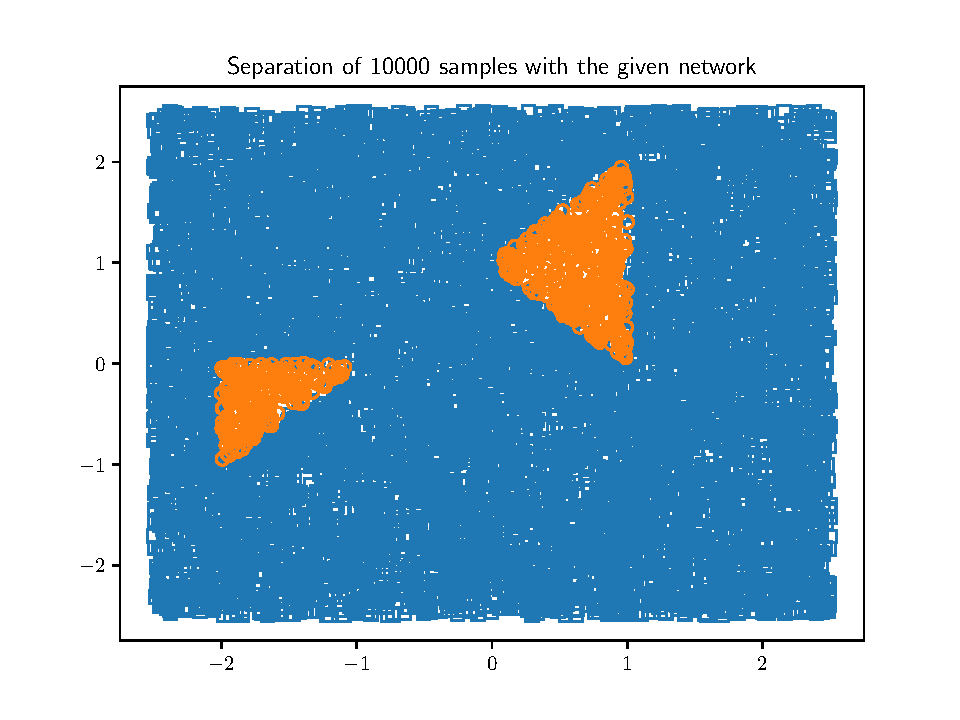
\includegraphics[width=.7\linewidth]{sep_10000.pdf}
\caption{Separation of 10000 samples with the given network}
\label{sep_10000}
\end{figure}

\section{Question 2}

\subsection{Complete Python code}

\lstinputlisting[basicstyle=\ttfamily\scriptsize]{hw2_ex2.py}

\end{document}